The infrastructure implemented for the experiments presented below is open
source and available online at \cite{sources}. The implementation is based on
TensorFlow \cite{abadi2015}, which is an efficient, flexible, and highly
scalable machine-learning library supported by all the major platforms including
the mobile ones.

The experiments are conducted on a \up{GNU}/Linux machine equipped with 8
\up{CPU}s Intel Core i7-3770 3.4~GHz, 16~\up{GB} of \up{RAM}, and an \up{HDD} of
500~\up{GB}. The machine has no modern \up{GPU}s; therefore, the reported
results have an immense room for improvement, which concerns not only timing but
potentially accuracy as well due to more extensive training.

\subsection{Data Processing}
Recall that the considered data set is the Google cluster-usage traces
\cite{reiss2011} described in \sref{data}. In the experiments, we focus on one
particular resource ($d = 1$), which is the \up{CPU} usage of the tasks executed
in the cluster. The resource-usage table contains two apposite columns: the
average and maximal CPU usage over five-minute intervals; we extract the former.

The grouping and indexing steps of the data-processing pipeline described in
\sref{grouping} and \sref{indexing}, respectively, and depicted in
\fref{workflow} take approximately 60 hours or 2--3 days (no parallelism). Since
they have to be done only once, their computational cost can be safely
considered negligible.

Regarding the selection stage delineated in \sref{selection}, we filter those
resource-usage traces that contain 5--50 data points; consequently, $l_i \in [5,
50]$ in \eref{trace}. Such traces constitute around 74\% of the total number of
traces (around 18 out of 24 million). We experiment with a random subset of two
million traces, which is around 11\% of the 5--50 resource-usage traces; hence,
$n = 2 \times 10^6$ in \eref{traces}. The data sets $X_1$, $X_2$, and $X_3$
constitute 70\%, 10\%, and 20\% of $X$, respectively. Fetching and storing on
disk these many traces take approximately four hours. Recall that this operation
has to be repeated only when the selection criteria change, which happens rarely
in practice.

\subsection{Modeling and Prediction}
The training stage (\sref{training}) is configured as follows. Ten buckets or
queues are used according to the following rule: $l < 6 < 7 < 8 < 9 < 10 < 15 <
20 < 30 < 40 \leq 50$. The batch size $b$ is set to 64. The optimization
algorithm employed for minimizing of the loss function is Adam
\cite{kingma2014}, which is an adaptive technique. The algorithm is utilized
with its default settings recommended by the algorithm's authors.

Regarding the validation stage (\sref{validation}), the considered
hyperparameters are the number of cells $c$ (the blue boxes in \fref{model}),
number of units per cell $u$ (the double circles in \fref{model}), and
probability of dropout $p$. More concretely, we let $c \in \{1, 2, 3, 4, 5\}$,
$u \in \{100, 200, 400, 800, 1600\}$, and $p \in \{0, 0.25, 0.5\}$, which yields
75 different combinations in total. The candidates are explored by means of the
Hyperband algorithm, which is introduced in \sref{validation}, with its default
settings. The maximum budget for one configuration is set to four training
epochs, which correspond to $4 \times 0.7 \times 2 \times 10^6 = 5.6 \times
10^6$ traces or $5.6 \times 10^6 \div 64 = 87\,500$ training steps.

The above exploration, which encompasses both the training and validation
stages, takes around 260 hours or 10--11 days. During this process, we run up to
four training sessions in parallel, which typically keeps all eight \up{CPU}s
busy. It should be noted that, due to the fact that the training, validation,
and testing data have been cached on disk as a result of our data-processing
pipeline described in \sref{data}, individual training sessions do not have any
overhead in this regard.

\begin{figure}[t]
  \centering
  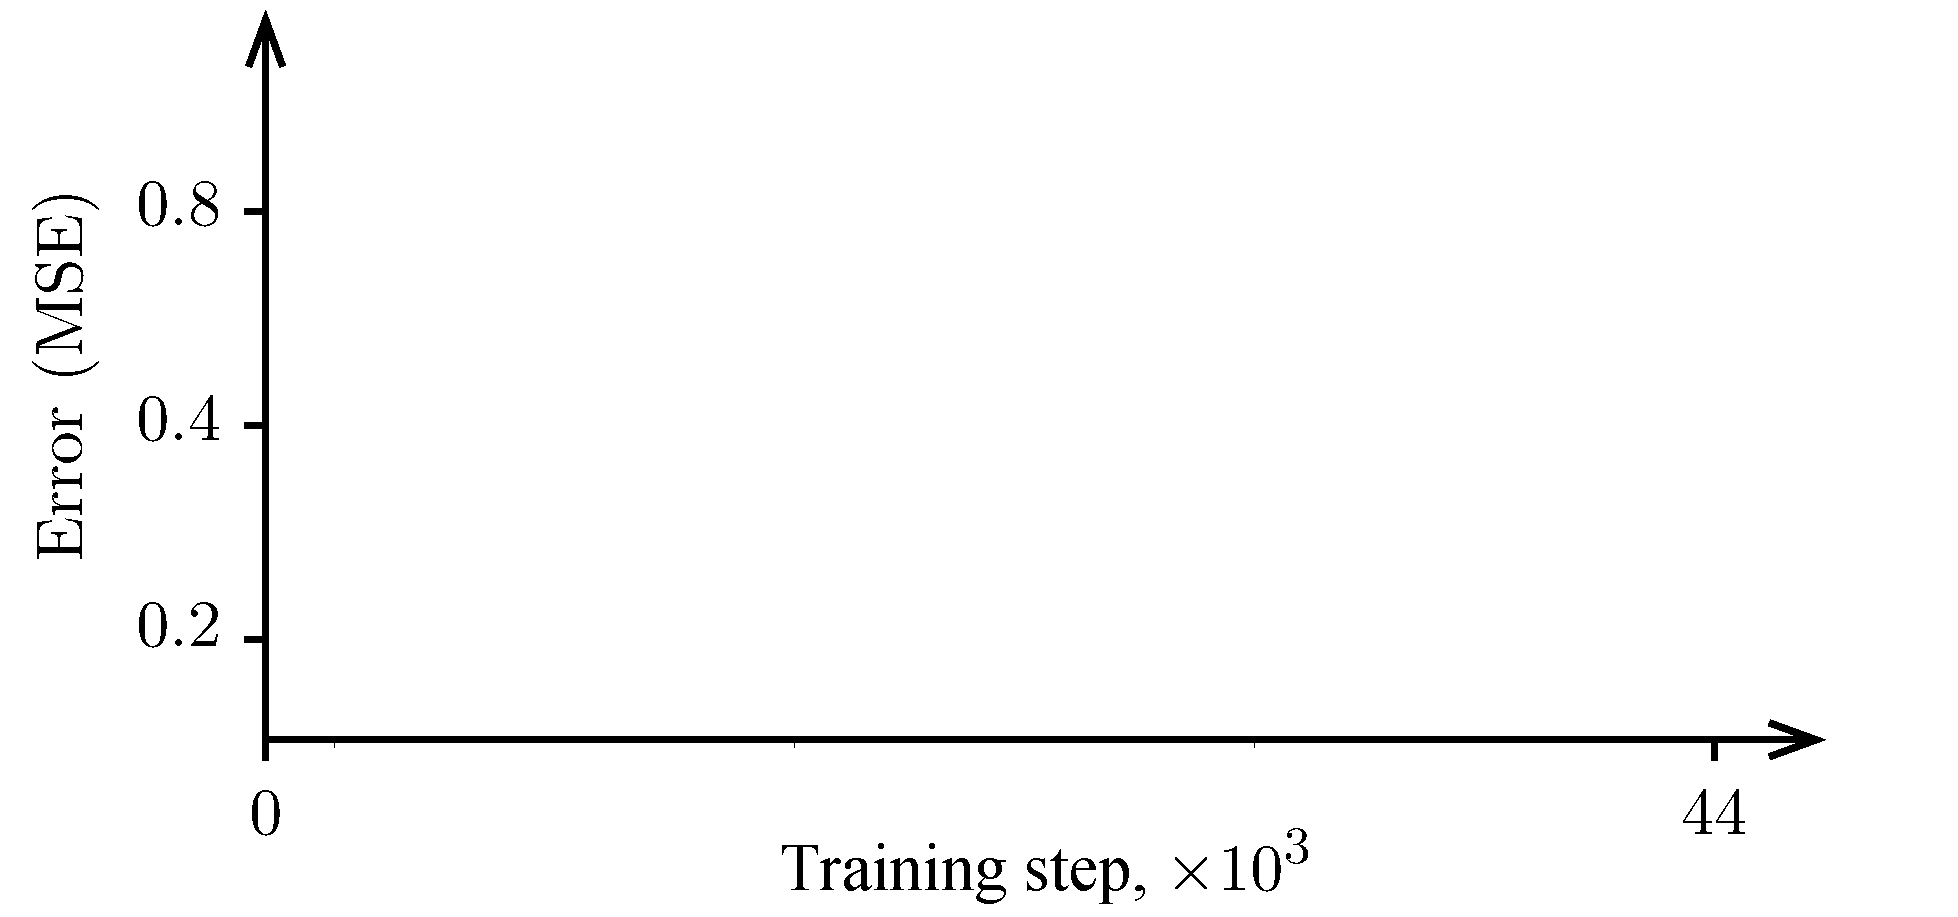
\includegraphics[width=1.0\columnwidth]{include/assets/figures/validation.pdf}
  \caption{
    The error of multiple configurations of hyperparameters with respect to the
    validation set $X_2$ while training using the training set $X_1$.
  }
  \vspace{-1.5em}
  \flab{validation}
\end{figure}

\begin{table}[b]
  \setlength{\tabcolsep}{4pt}
  \vspace{-2.0em}
  \caption{Validation results (top 10 configurations)}
  \vspace{-0.5em}
  \begin{tabular*}{\linewidth}{=L{30pt}-L{15pt}-R{25pt}-R{35pt}-R{50pt}-R{50pt}}
    \toprule
    Rank & $c$ & $u$ & $p$ & Error (\up{MSE}) & Memory (\up{MB}) \\
    \midrule
     1 & 3 & 1600 & 0.00 & 0.3148 & 198 \\
     2 & 4 & 1600 & 0.00 & 0.3154 & 277 \\
     3 & 3 & 1600 & 0.25 & 0.3158 & 198 \\
     4 & 2 &  800 & 0.25 & 0.3194 &  30 \\
     5 & 5 &  200 & 0.00 & 0.3205 &   6 \\
     6 & 2 & 1600 & 0.05 & 0.3207 & 119 \\
     7 & 5 &  800 & 0.00 & 0.3251 &  90 \\
     8 & 3 &  800 & 0.00 & 0.3257 &  50 \\
     9 & 1 & 1600 & 0.25 & 0.3278 &  40 \\
    10 & 2 &  800 & 0.00 & 0.3316 &  30 \\
    \bottomrule
  \end{tabular*}
  \tlab{validation}
\end{table}

The results of the validation stage are depicted in \fref{validation}, which
shows the mean squared error (\up{MSE}) of different configurations of the
hyperparameters as measured using $X_2$ ($0.1 \times 2 \times 10^6 = 2 \times
10^5$ traces). Note that only a subset of the candidates are shown since the
rest require a different scale and would render the figure illegible. Note also
how Hyperband operates: some of the sampled configurations are explored only
partially since they are regarded as less promising. The best trained model is
found to have the following hyperparameters: $c = 4$, $u = 1600$, and $p = 0$.
However, one can also observe in \fref{validation} that there are several other
candidates that are close to the best one. All these configurations correspond
to deeper and wider architectures, that is, to those that have more cells and
more units per cell (see \fref{model}). Finally, it is worth noting that the
curves readily plateau, which suggests a limit to what can be extracted from the
data with the model.

After the exploration stage, the best trained model is taken to the testing
stage (\sref{testing}), which is undertaken using $X_3$ ($0.2 \times 2 \times
10^6 = 4 \times 10^5$ traces). At this stage, the model is extensively assessed
by predicting the resource usage of individual tasks multiple time steps ahead
at each step of the testing traces in $X_3$. In these experiments, we predict
four steps into the future ($h = 4$ in \sref{problem}). This elaborate
sequential testing procedure takes around 15 hours from start to finish.

In order to assess better the accuracy of our resource-usage predictions, we
employ an alternative model, which we shall refer to as the reference model. The
reference model is based on random walk. It postulates that the best prediction
of what will happen tomorrow is what happens today: the next value of a
resource-usage trace is estimated to be the current one, which results in four
identical predictions at each time step.

The results of the testing stage can be seen in \fref{testing}, which shows the
\up{MSE} of our model (the blue line) as well as the one of the reference model
(the red line) with respect to $X_3$. The magnitude of our model's errors
suggests that the amount of regularity present in the data is not sufficient to
make the resource-usage predictions highly accurate. Nevertheless, it can be
seen in \fref{testing} that, relative to the reference model, our model provides
an error reduction of approximately 30\% at each of the four future time
moments. This observation indicates that a certain structure does exist, and
that it can be identified and utilized in order to make educated predictions.
